\documentclass[aspectratio=169]{beamer}
\usetheme[faculty=phil]{fibeamer}
\usepackage{polyglossia}
\setmainlanguage{english} %% main locale instead of `english`, you
%% can typeset the presentation in either Czech or Slovak,
%% respectively.
\setotherlanguages{russian} %% The additional keys allow
%%
%%   \begin{otherlanguage}{czech}   ... \end{otherlanguage}
%%   \begin{otherlanguage}{slovak}  ... \end{otherlanguage}
%%
%% These macros specify information about the presentation
\title[AGLA2]{Analytical Geometry and Linear Algebra II, Lab 1} %% that will be typeset on the
\subtitle{The geometry of linear equation\\
          Gaussian elimination\\
          Matrix notation and matrix multiplication} %% title page.
\author{Oleg Bulichev}
%% These additional packages are used within the document:
\usepackage{ragged2e}  % `\justifying` text
\usepackage{booktabs}  % Tables
\usepackage{tabularx}
\usepackage{tikz}      % Diagrams
\usetikzlibrary{calc, shapes, backgrounds}
\usepackage{amsmath, amssymb}
\usepackage{url}       % `\url`s
\usepackage{listings}  % Code listings
% \usepackage{subfigure}
\usepackage{floatrow}
\usepackage{subcaption}
\usepackage{todonotes}
\usepackage{fontspec}
\usepackage{multicol}
\graphicspath{{resources/}}
\frenchspacing

\setbeamertemplate{caption}[numbered]
\usetikzlibrary{graphs}

% \usepackage[backend=biber,style=ieee,autocite=footnote]{biblatex}
% \addbibresource{biblio.bib}
% \DefineBibliographyStrings{english}{%
%   bibliography = {References},}

\newcommand{\oleg}[2][] {\todo[color=red, #1] {OLEG:\\ #2}}
\newcommand{\fbckg}[1]{\usebackgroundtemplate{\includegraphics[width=\paperwidth]{#1}}}%frame background

\usepackage[framemethod=TikZ]{mdframed}
\newcommand{\dbox}[1]{
\begin{mdframed}[roundcorner=3pt, backgroundcolor=yellow, linewidth=0]
\vspace{1mm}
{#1}
\vspace{1mm}
\end{mdframed}
}

\begin{document}
\fbckg{fibeamer/figs/title_page.png}
\frame[c]{\setcounter{framenumber}{0}
    \usebeamerfont{title}%
    \usebeamercolor[fg]{title}%
    \begin{minipage}[b][6.5\baselineskip][b]{\textwidth}%
        \textcolor{black}{\raggedright\inserttitle}
    \end{minipage}
    % \vskip-1.5\baselineskip

    \usebeamerfont{subtitle}%
    \usebeamercolor[fg]{framesubtitle}%
    \begin{minipage}[b][3\baselineskip][b]{\textwidth}
      \raggedright%
      \insertsubtitle%
    \end{minipage}
    \vskip.25\baselineskip
}
%   \frame[c]{\maketitle}

\fbckg{fibeamer/figs/common.png}


% \section{Introduction}
% \begin{frame}[t]{\insertsectionhead}

\begin{frame}[t]{Task 1}
\framesubtitle{Warm up}
Rewrite the following system in the matrix form:
\begin{Large}
\begin{equation*}
    \left\{\begin{matrix}
       3x + 4y -2z = 1 \\ 
       3y -2z +x = -2 \\ 
       5x - 7z -2y = 3 
       \end{matrix}\right.
\end{equation*}
\end{Large}
\end{frame}

\begin{frame}[t]{Task 2}
\framesubtitle{}
    Describe geometricaly (line, plane, or whole space) all linear combinations of:
        \begin{enumerate}
            \item $\begin{bmatrix}1 \\ 2 \\3 \end{bmatrix}$ and $\begin{bmatrix}3 \\ 6 \\9 \end{bmatrix}$ \uncover<2-> {\alert{\textit{Ans}: line}}
            \item $\begin{bmatrix}1 \\ 0 \\0 \end{bmatrix}$ and $\begin{bmatrix}0 \\ 2 \\3 \end{bmatrix}$ \uncover<3-> {\alert{\textit{Ans}: plane}}
            \item $\begin{bmatrix}2 \\ 0 \\0 \end{bmatrix}$, $\begin{bmatrix}0 \\ 2 \\2 \end{bmatrix}$ and $\begin{bmatrix}2 \\ 2 \\3 \end{bmatrix}$ \uncover<4-> {\alert{\textit{Ans}: whole space}}
        \end{enumerate}
\end{frame}

\begin{frame}[c]{Task 3}
\framesubtitle{}\centering\large
    Draw $v = \begin{bmatrix}4 \\1 \end{bmatrix}$ and $w = \begin{bmatrix}-2 \\ 2 \end{bmatrix}$ and $ v + w $, $v-w$ in a single $xy$ plane
\end{frame}

\begin{frame}[t, label=task4]{Task 4}
\framesubtitle{}
    Explain, why the system is singular?
    \begin{equation*}
    \left\{\begin{matrix}
        u + v + w = 2 \\ 
        u + 2v + 3w = 1 \\ 
        v + 2w = 0 
        \end{matrix}\right.
    \end{equation*}

    What value should replace that last zero on the right side, to allow the equations to have solutions, and what is one of the solutions?
\end{frame}

\begin{frame}[t]{What does it mean, singular?}
\framesubtitle{Lec 1, page 11}
    \begin{figure}[H]
        \centering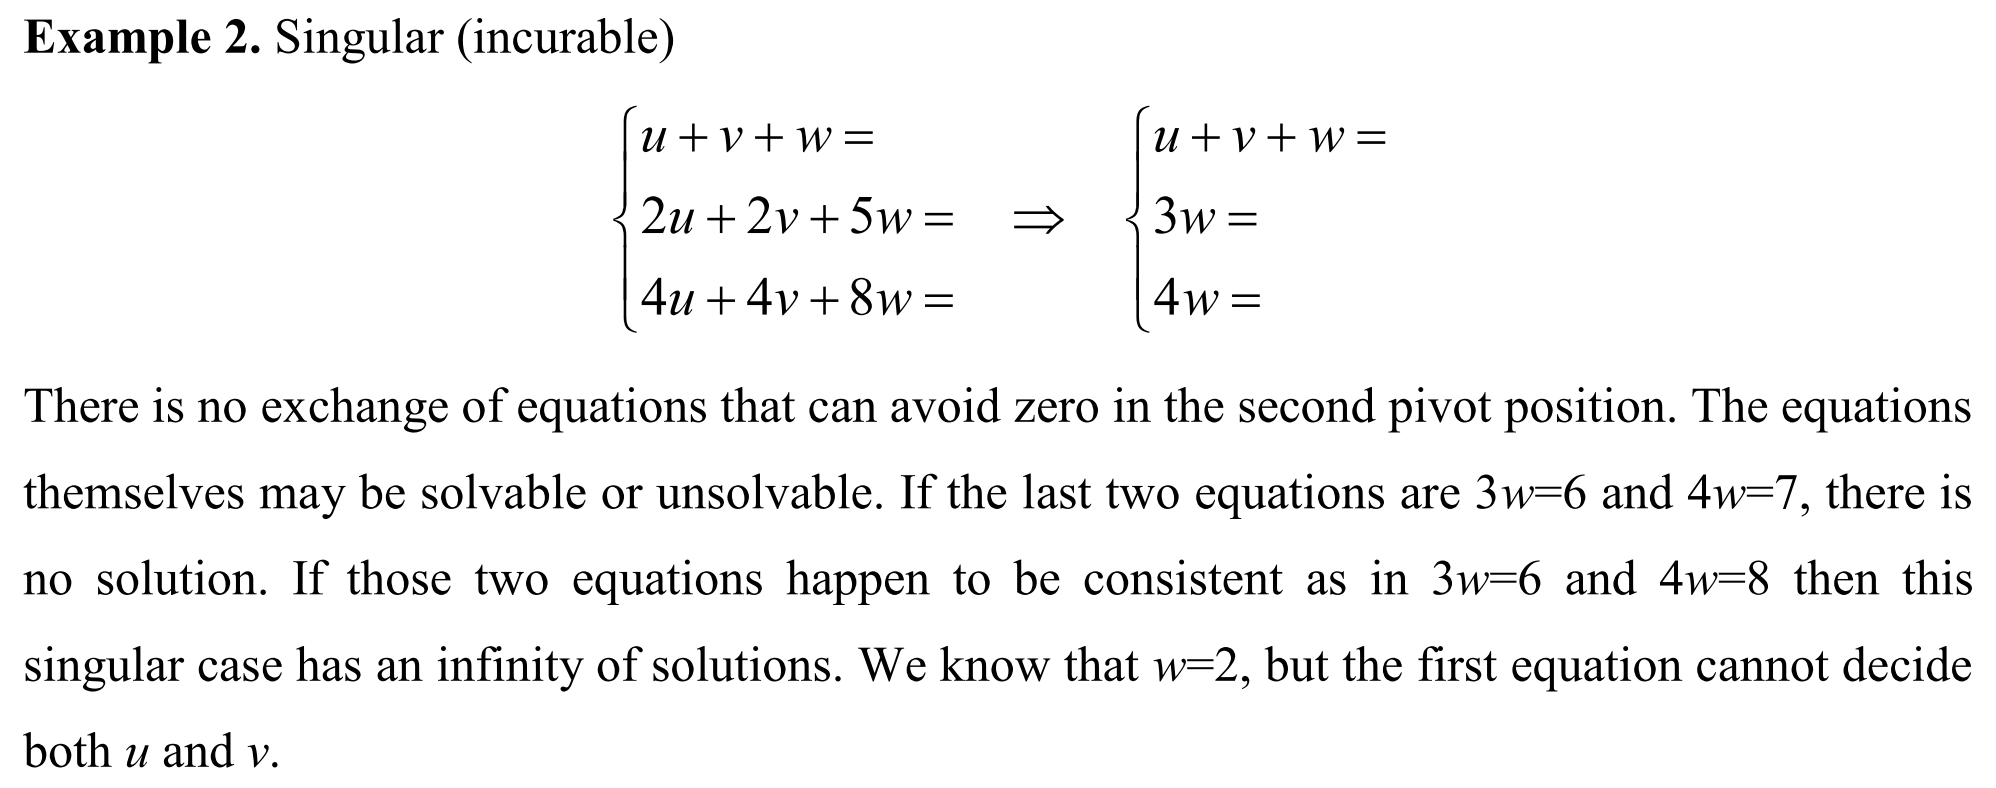
\includegraphics[height=6cm,width=1\textwidth,keepaspectratio]{1.png}
        % \caption{caption_name}
        \label{fig:1.png}
    \end{figure}
\end{frame}

\begin{frame}[t]{What does it mean, pivot point?}
\framesubtitle{}
    \Large
    \begin{definition}
        \textbf{The pivot or pivot element} is the element of a matrix, or an array, which is selected first on a particular step by an algorithm (e.g. Gaussian elimination, simplex algorithm, etc.), to do certain calculations.
    \end{definition}
\end{frame}

\againframe[t]{task4}

\begin{frame}[t]{Task 5}
\framesubtitle{}
    \begin{enumerate}
        \item Choose a coefficient $b$ that makes this system singluar.
        \item Then choose a right-hand side $g$ that makes it solvable.
        \item Find two solutions in that singular case.
    \end{enumerate}
    \begin{equation*}
        \left\{\begin{matrix}
            2x + by = 16 \\ 
            4x + 8y = g \\ 
            \end{matrix}\right.
    \end{equation*}    
\end{frame}

\begin{frame}[t]{Task 6}
\framesubtitle{}
    Give 3x3 examples (not just the zero matrix):
    \begin{enumerate}
        \item a diagonal matrix: $a_{ij}=0$, if $i \neq j$;
        \item a symmetric matrix: $a_{ij} = a_{ji}$ for all $i$ and $j$;
        \item an upper trianglular matrix: $a_{ij}=0$, if $i>j$ ;
        \item a skew-symmetric matrix: $a_{ij} = -a_{ji}$ for all $i$ and $j$.
    \end{enumerate}
\end{frame}

\begin{frame}<1>[t, label=task7]{Task 7}
\framesubtitle{}
    Obtain a Reduced Row Echelon Form (rref) of
    \begin{equation*}
        \left\{\begin{matrix}
            2u + 3v + 0w = 0 \\ 
            4u + 5v + w = 3 \\ 
            2u - 1v - 3w = 5 
            \end{matrix}\right.
        \end{equation*}
        \uncover<2>{\centering\alert{\textit{Ans}: $\left[\begin{array}{ccc|c}1 & 0 & 0 & 3 \\ 0 & 1 & 0 & -2 \\ 0 & 0 & 1 & 1\end{array}\right]$}}

\end{frame}

\begin{frame}[t]{The difference between REF and RREF}
\framesubtitle{}
\begin{block}{Gaussian elimination vs Gauss-Jordan elimination}
    \textbf{Gaussian elimination} refers to the process until it has reached its upper triangular.

    \textbf{Gauss-Jordan elimination} is the algorithm for converting a matrix into RREF.
\end{block}
The \textbf{Row Echelon Form} is \textit{not unique}
\vspace{-7pt}
    \begin{equation*}
        \begin{bmatrix} 1 & 3 & -1 \\ 0 & 1 & 7 \\ \end{bmatrix} 
        \xrightarrow{\text{add row 2 to row 1}}
        \begin{bmatrix} 1 & 4 & 6 \\ 0 & 1 & 7 \\ \end{bmatrix}. 
    \end{equation*}
   Every matrix has a \textit{ unique} \textbf{Reduced Row Echelon Form}
\vspace{-7pt} 
   \begin{equation*}
        {\displaystyle {\begin{bmatrix}1&3&-1\\0&1&7\\\end{bmatrix}}{\xrightarrow {\text{subtract 3 × (row 2) from row 1}}}{\begin{bmatrix}1&0&-22\\0&1&7\\\end{bmatrix}}.}
    \end{equation*}
\end{frame}

\againframe<2>[t]{task7}

\begin{frame}[t]{Reference material}
\framesubtitle{}
\Large
    \begin{itemize}
        \item \href{https://ocw.mit.edu/courses/mathematics/18-06-linear-algebra-spring-2010/video-lectures/}{Lectures 1 -- 3}
    \end{itemize}
\end{frame}


\fbckg{fibeamer/figs/last_page.png}
\frame[plain]{}

\end{document}